\documentclass[12pt]{article}
\usepackage{fullpage}
\usepackage{lastpage}
\usepackage{fancyhdr}
\pagestyle{fancy}

\addtolength{\topmargin}{-0.25in}
\usepackage{graphicx}	
\usepackage{array, multicol}
\usepackage{amsmath}
\usepackage{comment}
\usepackage{enumerate}
\usepackage{url}

\everymath{\displaystyle}

\fancypagestyle{plain}{
	\fancyhf{}
	\addtolength{\headheight}{2.92\baselineskip}
	\lhead{\bf MATH 2554 (Calculus I) \\
		Summer 2015 \\
		}
	\rhead{{Name:} \underline{\hspace{40ex}} \\
		\vspace{0.5pc}
		Thurs 2 July 2015}
	\rfoot{%Exam 3A 
	Exam 3B
	p.\thepage\ (of \pageref{LastPage})}
	}
\fancyhf{}
\renewcommand{\headrulewidth}{0pt}

\title{\vspace{-8pc}
\vfill{\Huge
	\bf Exam 3: Using Derivatives ($\textstyle\oint$3.10-4.6)} \\
	%Version A
	Version B
	}
\author{}
\date{}

\rfoot{%Exam 3A 
	Exam 3B
	p.\thepage\ (of \pageref{LastPage})}

% % % % %
\begin{document}
\maketitle
\vspace{-3pc}
\noindent{\bf Exam Instructions:} You have 50 minutes to complete this exam.  Follow the directions and answer the question, using boss notation where appropriate.  Justification is required for all problems. 

\vspace{2pc}
\noindent\textbf{Your signature below indicates that you have read this page and agree to follow the Academic Honesty Policies of the University of Arkansas.}  

\vfill
\noindent Signature: {\bf (1 pt)} \underline{\hspace{73ex}}
\begin{flushright}\Large Good luck!\end{flushright}

\newpage
\begin{enumerate}
% % % % %
\begin{comment} % Version A
\item {\bf (20 pts)} Sketch a graph of a function $f(x)$, continuous on $(-\infty,\infty)$, that satisfies all of the following criteria:
\begin{itemize}
\item $f(-2)=f(2)=0$
\item $f^{\prime}(x)>0$ and $f^{\prime\prime}(x)>0$ on $(-\infty,-2)$
\item $f^{\prime}(x)>0$ and $f^{\prime\prime}(x)<0$ on $(-2,0)$
\item $f^{\prime}(x)<0$ and $f^{\prime\prime}(x)<0$ on $(0,2)$
\item $f^{\prime}(x)=0$ on $(2,\infty)$
\end{itemize}
\end{comment}
%
%\begin{comment} % Version B
\item {\bf (20 pts)} Sketch a graph of a function $f(x)$, continuous on $(-\infty,\infty)$, that satisfies all of the following criteria:
\begin{itemize}
\item $f(-4)=1$ and $f(2)=-1$
\item $f^{\prime}(x)<0$ and $f^{\prime\prime}(x)<0$ on $(-\infty,0)$
\item $f^{\prime}(x)<0$ and $f''(x)>0$ on $(0,2)$
\item $f^{\prime}(x)>0$ and $f^{\prime\prime}(x)>0$ on $(2,4)$
\item $f^{\prime}(x)>0$ and $f^{\prime\prime}(x)<0$ on $(4,\infty)$
\end{itemize}
%\end{comment}

% % %
\newpage
\item \begin{enumerate}
	\item {\bf (9 pts)} What are the three hypotheses for Rolle's Theorem?
	\vspace{9pc}
	
	\item {\bf (7 pts)} Given the three hypotheses, what is the conclusion of Rolle's Theorem?
	\vspace{7pc}
	
	\item {\bf (7 pts)} The \emph{Mean Value Theorem} applies to 
	%$f(x)=x(x^2+x+2)$ % Version A
	$f(x)=x(x^2-x-2)$ %Version B
	on $[-1,1]$.  (You don't have to prove that.)  Find the point(s) guaranteed to exist by the Mean Value Theorem.   
	\end{enumerate}

% % %
\newpage
\item {\bf (7 pts ea)} Let 
	%$f(x)=\ln x + \sin{(2-x)}$. % Version A
	$f(x)=\ln x - \sin{(2-x)}$. % Version B
	\begin{enumerate}
	\item Write the equation for the linear approximation to $f(x)$ at $x=2$.
	\vspace{12pc}
	
	\item Use your answer to (a) to approximate $f(1)$.
	\vspace{4pc}
	
	\item Below is the graph of $f(x)$, drawn at the website \url{desmos.com/calculator}. On the same axis, draw your tangent line.  Label both $f(1)$ and your approximation from part (b).
	\vspace{2pc}
	
	%\centering{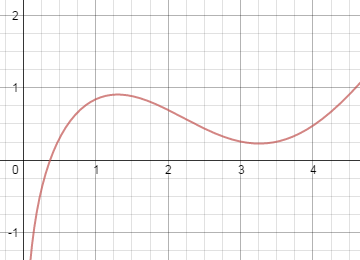
\includegraphics[scale=1.25]{exam3asec4p5}} % Version A
	\centering{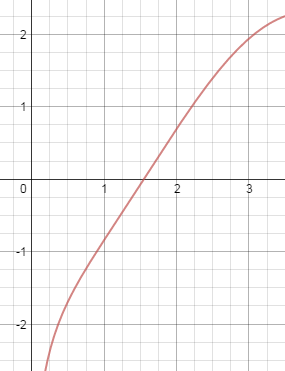
\includegraphics[scale=1]{exam3bsec4p5}} % Version B
	\end{enumerate}
	
% % %
\newpage
%\item {\bf (20 pts)} A landscaper wants to make a rectangular flower garden with an area of 24 in$^{\text{2}}$, surrounded by 6 in of rocks on either side and 1 in of astroturf above and below.  What dimensions of the garden will minimize the combined area of the garden with its rocks and astroturf borders?  Use the 2nd Derivative Test to justify your answer. % Version A
%
\item {\bf (20 pts)} A rectangular flower garden with an area of 32 $\text{m}^2$ is surrounded by a grass border that is 1 m wide on the top and bottom, and 2 m wide on the other two sides.  What dimensions of the garden minimize the combined area of the garden and borders?  Use the 2nd Derivative Test to justify your answer.  % Version B  

% % %
\newpage
\item {\bf (10 pts ea)} Let $f(x)$ be a function, continuous on $(-\infty,\infty)$, such that 
\[
%f^{\prime}(x)=\frac{2-2x^2}{(1+x^2)^2} % Version A 
f^{\prime}(x)=\frac{2-2x^2}{1+x^2} % Version B 
\quad\text{and}\quad 
%f^{\prime\prime}(x)=\frac{6x^3-10x}{(1+x^2)^3}. % Version A
f^{\prime\prime}(x)=\frac{-8x}{(1+x^2)^2}. % Version B
\]
\begin{enumerate}
	\item Determine the intervals on which $f(x)$ is increasing and decreasing.
	\vspace{14pc}

	\item Determine the intervals on which $f(x)$ is concave up and concave down.
\end{enumerate}

% % %
\newpage
%\item {\bf (20 pts)} A rectangle initially has dimensions 2 cm by 4 cm.  All sides begin increasing in length at a rate of 1 cm/sec.  At what rate is the area of the rectangle increasing after 20 sec? % Version A
%
\item {\bf (20 pts)} A rectangle initially has dimensions 1 cm by 5 cm.  All sides begin increasing in length at a rate of 2 cm/sec.  At what rate is the area of the rectangle increasing after 20 sec? % Version B

% % % % %
\end{enumerate}
\end{document}